\documentclass[a4paper,11pt]{report}

\usepackage{amsmath,amssymb}
\usepackage{fullpage}
\usepackage{graphicx}
\usepackage[cache=false]{minted}

\usepackage{bussproofs}
\usepackage{mathpartir}
\usepackage{prooftrees}
\usepackage{color}

\usepackage{tikz}
\usetikzlibrary{automata,positioning}

\newcommand*\circled[1]{\tikz[baseline=(char.base)]{
            \node[shape=circle,draw,inner sep=2pt] (char) {#1};}}

\makeatletter
\pgfmathdeclarefunction{alpha}{1}{%
  \pgfmathint@{#1}%
  \edef\pgfmathresult{\pgffor@alpha{\pgfmathresult}}%
}

\newcommand*{\until}{U}
\newcommand*{\disj}{\ ,\ }
\newcommand*{\A}{\square}  % Always
\newcommand*{\D}{\diamondsuit} % eventually

\newcommand*{\Pq}{(\top,\bot)}
\newcommand*{\pQ}{(\bot,\top)}
\newcommand*{\PQ}{(\top,\top)}
\newcommand*{\pq}{(\bot,\bot)}

\usemintedstyle{tango}

\newminted[promelacode]{C}{
  frame=single,
  framesep=6pt,
  breaklines=true,
  fontsize=\scriptsize
}

\newmintinline[promelainline]{C}{breaklines=true,fontsize=\small}

\newmintedfile{c}{frame=single, framesep=6pt, breaklines=true,fontsize=\scriptsize}
\newcommand{\ex}[3]{\cfile[firstline=#1,lastline=#2]{ex#3.pml}}

% tikz
\usepackage{tikz}
\usetikzlibrary{snakes}

\author{Sylvain Julmy}
\date{\today}

\setlength{\parindent}{0pt}
\setlength{\parskip}{2.5pt}

\begin{document}

\begin{center}
\Large{
    Verification of Cyber-Physical System\\
    Fall 2017
  }
  
  \noindent\makebox[\linewidth]{\rule{\linewidth}{0.4pt}}
  Exercice Sheet 5

  \vspace*{1.4cm}

  Author : Sylvain Julmy
  \noindent\makebox[\linewidth]{\rule{\linewidth}{0.4pt}}

  \begin{flushleft}
    Professor : Ultes-Nitsche Ulrich
    
    Assistant : Prisca Dotti
  \end{flushleft}

  \noindent\makebox[\linewidth]{\rule{\textwidth}{1pt}}
\end{center}

\section*{Exercice 1}

\subsection*{(1)}

Local automata :

\begin{center}
  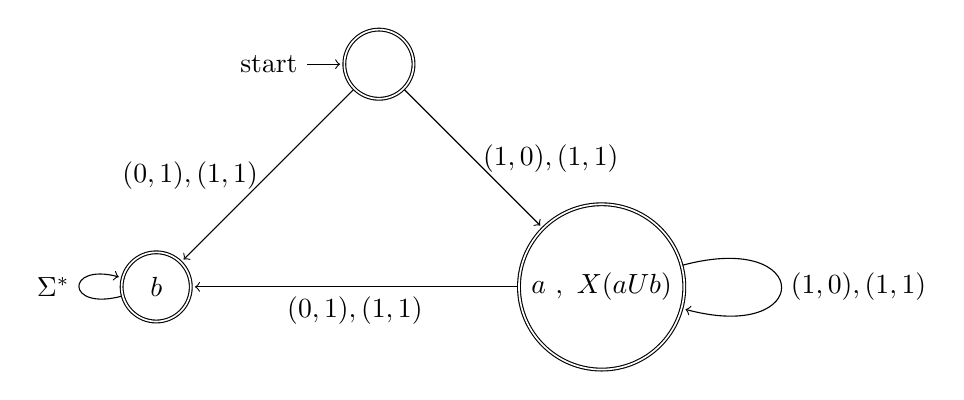
\begin{tikzpicture}[shorten >=1pt,node distance=4cm,on grid,auto]
    \node[state,initial,accepting] (init) {};
    \node[state,accepting] (b) [below left = of init] {$b$};
    \node[state,accepting] (a) [below right = of init] {$a \disj X(a\until b)$};
    \path[->]
    (init)
    edge node [left] {$(0,1),(1,1)$} (b)
    edge node [right] {$(1,0),(1,1)$} (a)
    (b)
    edge [loop left] node {$\Sigma^*$} ()
    (a)
    edge node {$(0,1),(1,1)$} (b)
    edge [loop right] node {$(1,0),(1,1)$} ()
    ;
  \end{tikzpicture}
\end{center}

We use some annotation in order to simplify the readings :

\begin{center}
  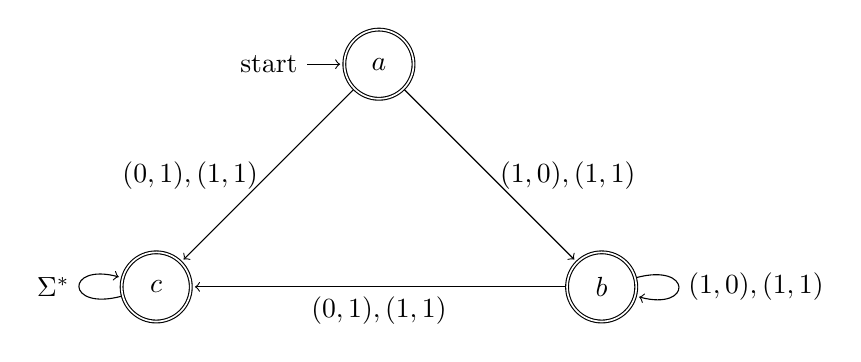
\begin{tikzpicture}[shorten >=1pt,node distance=4cm,on grid,auto]
    \node[state,initial,accepting] (init) {$a$};
    \node[state,accepting] (b) [below left = of init] {$c$};
    \node[state,accepting] (a) [below right = of init] {$b$};
    \path[->]
    (init)
    edge node [left] {$(0,1),(1,1)$} (b)
    edge node [right] {$(1,0),(1,1)$} (a)
    (b)
    edge [loop left] node {$\Sigma^*$} ()
    (a)
    edge node {$(0,1),(1,1)$} (b)
    edge [loop right] node {$(1,0),(1,1)$} ()
    ;
  \end{tikzpicture}
\end{center}

Eventuality automata :

\begin{center}
  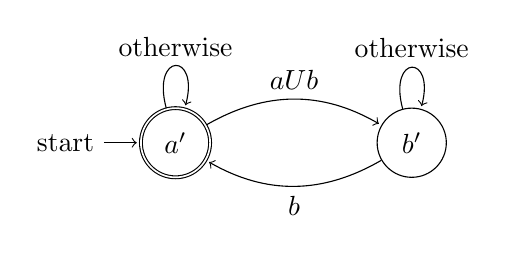
\begin{tikzpicture}[shorten >=1pt,node distance=3cm,on grid,auto]
    \node[state,initial,accepting] (a) {$a'$};
    \node[state] (b) [right = of a] {$b'$};
    \path[->]
    (a)
    edge [bend left] node {$a \until b$} (b)
    edge [loop above] node {otherwise} ()
    (b)
    edge [bend left] node {$b$} (a)
    edge [loop above] node {otherwise} ()
    ;
  \end{tikzpicture}
\end{center}

Complete automaton :

\begin{center}
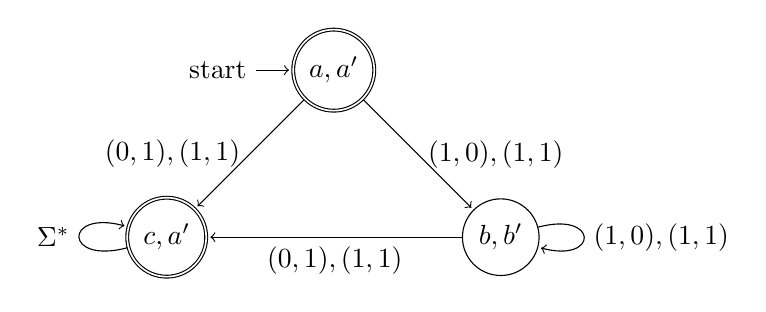
\begin{tikzpicture}[shorten >=1pt,node distance=3cm,on grid,auto]
    \node[state,initial,accepting] (init) {$a,a'$};
    \node[state,accepting] (b) [below left = of init] {$c,a'$};
    \node[state] (a) [below right = of init] {$b,b'$};
    \path[->]
    (init)
    edge node [left] {$(0,1),(1,1)$} (b)
    edge node [right] {$(1,0),(1,1)$} (a)
    (b)
    edge [loop left] node {$\Sigma^*$} ()    
	(a)
    edge node {$(0,1),(1,1)$} (b)
    edge [loop right] node {$(1,0),(1,1)$} ()
    ;
  \end{tikzpicture}
\end{center}

\subsection*{(2)}

First, we transform

\[
  \square \diamondsuit a
\]

into

\begin{align*}
  \square \diamondsuit a &\equiv \neg \diamondsuit \neg (\diamondsuit a) \\
                         &\equiv \neg (\top \until (\neg (\diamondsuit a))) \\
                         &\equiv \neg (\top \until(\neg(\top \until a)))
\end{align*}

Algorithmic sugar (note : we simplify formulae like $\top \wedge a \equiv a$ and
$\bot \vee a \equiv a$) :

\begin{center}
  \begin{forest}
    [$ \neg (\top \until(\neg(\top \until a)))$
    [$ \neg (\neg \top \until a) \wedge (\neg \top \vee \neg X(\top \until (\neg(\top \until a))))$
    [$ \neg (\neg \top \until a) \disj (\neg \top \vee \neg X(\top \until (\neg(\top \until a))))$
    [$ \top \until a \disj \bot \vee \neg X(\top \until (\neg(\top \until a)))$
    [$ a \vee (\top \wedge X(\top \until a)) \disj \bot \vee \neg X(\top \until (\neg(\top \until a)))$
    [$a \disj \neg X(\top \until (\neg(\top \until a)))$
    [\fbox{$a \disj X(\neg(\top \until (\neg (\top \until a)))) $}
    [$\neg(\top \until (\neg (\top \until a)))$ [$\cdots$]]]
    ]
    [$ X(\top \until a) \disj \neg X(\top \until (\neg(\top \until a)))$
    [\fbox{$X(\top \until a) \disj X(\neg(\top \until (\neg (\top \until a))))$}
    [$\neg(\top \until (\neg (\top \until a)))$ [$\cdots$]]]
    ]    ]    ]    ]    ]    ]    ]
  \end{forest}
\end{center}

Eventuality automaton for ($\top \until a$)

\begin{center}
  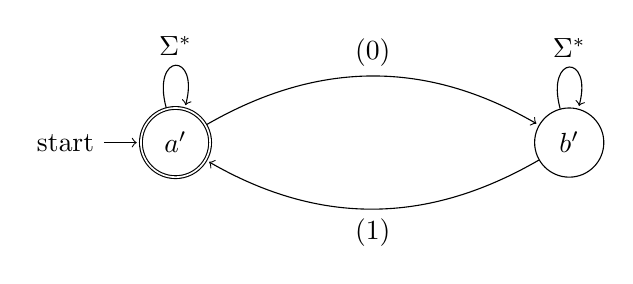
\begin{tikzpicture}[shorten >=1pt,node distance=5cm,on grid,auto]
    \node[state,accepting,initial] (q0) {$a'$};
    \node[state] (q1) [right = of q0] {$b'$};
    \path[->]
    (q0)
    edge [loop above] node {$\Sigma^*$} ()
    edge [bend left] node {$(0)$} (q1)
    (q1)
    edge [loop above] node {$\Sigma^*$} ()
    edge [bend left] node {$(1)$} (q0)
    ;
  \end{tikzpicture}
\end{center}

Local automaton :

\begin{center}
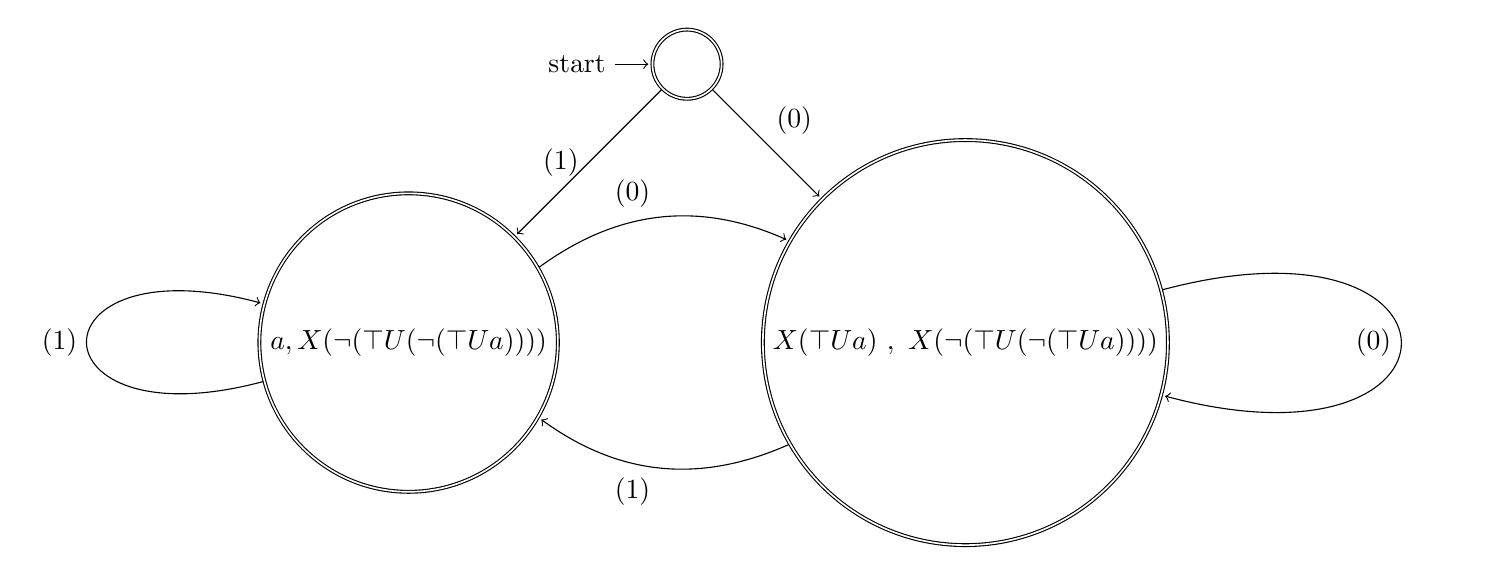
\begin{tikzpicture}[shorten >=1pt,node distance=5cm,on grid,auto]
    \node[state,initial,accepting] (init) {};
    \node[state,accepting] (a) [below left = of init] {$a,X(\neg (\top \until (\neg (\top \until a))))$};
    \node[state,accepting] (b) [below right = of init] {$X(\top \until a) \disj X(\neg(\top \until (\neg (\top \until a))))$};
    \path[->]
    (init)
    edge node[left] {$(1)$} (a)
    edge node {$(0)$} (b)
    (a)
    edge [bend left] node {$(0)$} (b)
    edge [loop left] node {$(1)$} ()
    (b)
    edge [bend left] node {$(1)$} (a)
    edge [loop right] node [left] {$(0)$} ()    
	;
  \end{tikzpicture}
\end{center}

Complete automaton
\begin{center}
  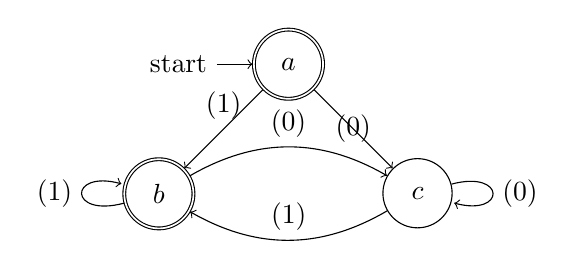
\begin{tikzpicture}
    \node[state,initial,accepting] (init) {$a$};
    \node[state,accepting] (a) [below left = of init] {$b$};
    \node[state] (b) [below right = of init] {$c$};
    \path[->]
    (init)
    edge node[above] {$(1)$} (a)
    edge node {$(0)$} (b)
    (a)
    edge [bend left] node [above] {$(0)$} (b)
    edge [loop left] node {$(1)$} ()
    (b)
    edge [bend left] node [above] {$(1)$} (a)
    edge [loop right] node {$(0)$} ()    
    ;
  \end{tikzpicture}
\end{center}

\section*{Exercice 2}

\subsection*{(1)}
\[
  \A \D (x == 1)
\]

It is not a safety property, because it does not exist a finite execution of the
system that would not satisfies this formula, because we always need to ``know''
if $x==1$ or not in order to unvalidate the property.

It is a liveness property, because the property is checking, at any moment, if
$x==1$ would occurs now or in the future.

\subsection*{(2)}
\[
  \neg (\A \D (x < 36))
\]

It is not a safety property, because it does no exist a finite execution of the
system that would not satisfies the formula. For example, if $x < 36$ occurs $2$
times, we don't know if the property would hold or not in the future.

It is a liveness property, we could transform the formula to $\neg (\A \D (x <
36)) = \neg (\neg (\D \neg (\D (x < 36)))) = \D \neg (\D (x < 36))$, and here
the property would check if $\D (x < 36)$ would not happen.

\subsection*{(3)}
\[
  \D (\neg (x > 10))
\]

It is a liveness property, we check if $\neg(x > 10)$ would eventually happen or
not. We could transform $\neg(x > 10)$ to $x \leq 10$, and $\D (x \leq 10)$ is a
liveness property.

It is not a safety property, because it is a liveness property.

\subsection*{(4)}
\[
  \neg\D(x == 12)
\]

It is a safety property, because it exist a finite execution of the system that
does not satisfy this property, for example if $x==12$ now, the property does
not hold and any further execution of the system would satisfies the property.

It is not a liveness property, because it is a safety property.

\end{document}